\begin{center}
\begin{tabular}{|c|}
\hline
\begin{large} secHA1LosC \end{large}\\
\hline
Losa. Tramo Central. Sección normal al eje X.\\
\hline
\begin{tabular}{c|l}
\begin{minipage}{85mm}
\vspace{2mm}
\begin{center}
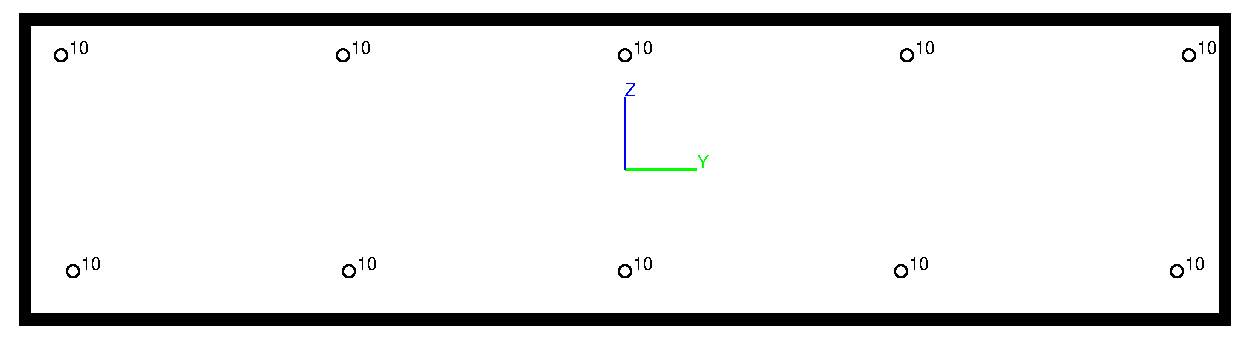
\includegraphics[width=80mm]{seccion.eps}
\end{center}
\vspace{1pt}
\end{minipage} & 
\begin{tabular}{l}
ancho: \\
$b= 1.00\ m$\\
canto: \\
$h= 0.25\ m$\\
\end{tabular} \\
\end{tabular} \\
\hline
\textbf{Materiales}:\\
\hline
\begin{tabular}{ll}
Hormigón: HA25 & Módulo de deformación longitudinal: $E_c= 27.26\ GPa$\\
\hline
Acero: B500S & Módulo elástico: $E_s= 200.00\ GPa$\\
\end{tabular} \\
\hline
\textbf{Valores estáticos}:\\
\hline
Sección bruta:\\
\hline
\begin{tabular}{ll}
$A_{bruta}= 0.250\ m^2$ & \multirow{3}{*}{Tensor de inercia ($cm^4$): $ \left( \begin{array}{ccc}43.91 & 0.00 & 0.00 \\ 0.00 & 13.02 &  0.00 \\ 0.00 &  0.00 & 208.33 \end{array} \right)$} \\
& \\
C.D.G.: $( 0.00, 0.00)\ m$  & \\
\end{tabular} \\
\hline
Sección homogeneizada:\\
\hline
\begin{tabular}{ll}
$A_{homog.}= 0.257\ m^2$ & \multirow{3}{*}{Tensor de inercia ($cm^4$): $ \left( \begin{array}{ccc}43.91 & 0.00 & 0.00 \\ 0.00 & 13.63 &  0.00 \\ 0.00 &  0.00 & 216.37 \end{array} \right)$} \\
& \\
C.D.G.: $( 0.00, 0.00)\ m$  & \\
\end{tabular} \\
\hline
\textbf{Armadura pasiva}:\\
\hline
\begin{tabular}{ll}
Área total $A_s= 7.90\ cm^2$ & Cuantía geométrica $\rho= 3.16\permil$\\
\end{tabular} \\
\hline
Familias de armadura principal:\\
\hline
\begin{tabular}{cccccccc}
Id & n. barras & $\phi$ & área & c. geom. & recub. mec. & $y_{cdg}$ & $z_{cdg}$\\
 &  & $(mm)$ & $(cm^2)$ & $(\permil)$ & $(cm)$ & $(m)$ & $(m)$\\
\hline
neg & 5 & 10 &  3.95 & 1.58 &  4.0 & -0.000 & -0.085\\
\hline
pos & 5 & 10 &  3.95 & 1.58 &  3.0 & -0.000 & 0.095\\
\end{tabular} \\
\hline
Familias de armadura de cortante:\\
\hline
\begin{tabular}{cccccccc}
Id & n. ramas & $\phi$ & área & sep. & area/m & $\alpha$ & $\beta$\\
 &  & $(mm)$ & $(cm^2)$ & $(cm)$ & $(cm^2/m)$ & $( \degree)$ & $( \degree)$\\
\hline
Vz & 4 & 6 &  1.12 & 20.0 &  5.60 & 90.0 & 45.0\\
\hline
Vy & 2 & 6 &  0.56 & 20.0 &  2.80 & 90.0 & 45.0\\
\end{tabular} \\
\hline
\end{tabular}
\end{center}
